\documentclass{article}
\usepackage{natbib}
\usepackage{color}
\usepackage[dvipsnames,svgnames*]{xcolor}
\usepackage{array}
\usepackage[colorlinks=TRUE, linkcolor=blue]{hyperref}
\usepackage{wrapfig,float}
\usepackage[font=small,skip=5pt]{caption}
\usepackage[aboveskip=2pt]{subcaption}
\usepackage{graphicx}
\usepackage{amsmath}
\usepackage{dsfont}
\usepackage{amsthm}
\usepackage{amsfonts}
\usepackage{url}
\usepackage{ulem}
\usepackage[section]{placeins}
\usepackage{afterpage}
\usepackage{bbm}
\usepackage{Sweave}
\begin{document}
\Sconcordance{concordance:ar1_predictive.tex:ar1_predictive.Rnw:%
1 19 1 1 0 129 1 1 73 4 1 1 63 1 1 1 6 1 2 5 1}


We have $T$ observations from an AR(1) model:

$$y_{t} = \mu + \psi y_{t-1}+ \epsilon_{t},$$

Where $\epsilon_{t}$ is $iid \hspace{4pt} \mathcal{N}(0,\sigma^2).$

We use $y_1 \sim \mathcal{N}(0, \tau^2)$, which results in the vector $y_{1:T}$ having the likelihood function

\begin{eqnarray*}
\label{likelihood}
L(\mu, \psi, \sigma | y_{1:T}, \tau) & = & \mathcal{N}(0, \tau) \prod_{t=2}^{T} \mathcal{N}(\mu + \psi y_{t-1}, \sigma^2) \nonumber \\
& = & \frac{1}{(2\pi)^T} \tau^{-1} \exp \left\{ \frac{-y_1^2}{2\tau^2}\right\} \sigma^{-(T-1)} \exp \left\{ \frac{-\sum^{T}_{t=2}(y_t-(\mu+\psi y_{t-1}))}{2\sigma^2}\right\}  
\end{eqnarray*}

We restrict $\psi$ to $(0, 1)$ and use the priors:
\begin{eqnarray*}
\label{priors}
p(\mu) & \propto & 1 \\
p(\sigma^2) & \propto & \sigma^{-2} \\
p(\psi) & \sim & \mathcal{B}(p1, p2).
\end{eqnarray*}



We get a joint distribution
\begin{eqnarray*}
\label{joint}
p(y_{1:T}, \mu, \psi, \sigma^2) & \propto &  \tau^{-1} \sigma^{-(T-1)}  \exp \left\{ \frac{-y_1^2}{2\tau^2}\right\} \exp \left\{ \frac{-\sum^{T}_{t=2}(y_t-(\mu+\psi y_{t-1}))^2}{2\sigma^2}\right\} \psi^{p1-1}(1-\psi)^{p2-1}
\end{eqnarray*}

However, we are interested in the forecast distribution of $y_{T+1}$, where $p(y_{T+1} | \mu, \psi, \sigma^2, y_T) \sim \mathcal{N}(\mu + \psi y_T, \sigma^2).$

Incorporating this into the above results in
\begin{eqnarray*}
\label{jointpred}
p(y_{1:T+1}, \mu, \psi, \sigma^2) & \propto &  \tau^{-1} \sigma^{-(T-2)}  \exp \left\{ \frac{-y_1^2}{2\tau^2}\right\} \exp \left\{ \frac{-\sum^{T}_{t=2}(y_t-(\mu+\psi y_{t-1}))^2}{2\sigma^2}\right\} \\
& \times &  \psi^{p1-1}(1-\psi)^{p2-1} \exp \left\{ \frac{-(y_{T+1}-(\mu+\psi y_T))^2}{2\sigma^2} \right\} \\
\ln(p(y_{1:T+1}, \mu, \psi, \sigma^2)) & = & -\ln(\tau) - (T-2) \ln(\sigma) - \frac{y_1^2}{2\tau^2} - \frac{\sum^{T}_{t=2}(y_t-(\mu+\psi y_{t-1}))^2}{2\sigma^2} \\
& - &  \frac{(y_{T+1}-(\mu+\psi y_T))^2}{2\sigma^2} + (p_1-1) \ln(\psi) + (p_2-1)\ln(1-\psi).
\end{eqnarray*}

We use the factorisation $q(\mu, \psi, \sigma^2, y_{T+1}) = q(\mu)q(\psi)q(\sigma^2)q(y_{T+1})$ in the variational bayes approximation.

It can be shown that the approximations that minimise the KL Divergence between the true posterior and the approximation is of the form
$$q_{\theta_i} \propto \exp(E_{q_{\theta_{\setminus i}}} (\ln(p(y,\theta)))) \mbox{ for i = 1,2, \dots}$$
where the notation $\theta_{\setminus i}$ refers to all $\theta$ except $\theta_i$.

Proceeding by taking the expectation of the log joint distribution with respect to all terms but $\mu$, and ignoring all terms that do not depend on $\mu$ we have

\begin{eqnarray*}
\label{qmu}
\ln(q(\mu)) & = & \mathbb{E}_{\psi, \sigma^2, y_{T+1}} \left[ \frac{-1}{2\sigma^2} \left(\sum^{T}_{t=2}(y_t-(\mu+\psi y_{t-1})) + (y_{T+1}-(\mu+\psi y_T))^2 \right) \right] + c \\
& = &  \mathbb{E}_{\sigma^2} \left[ \frac{-1}{2\sigma^2} \right] \mathbb{E}_{\psi, y_{T+1}} \Bigg[ \sum^{T}_{t=2} (y_t^2 + (\mu+\psi y_{t-1})^2 - 2 y_t (\mu+\psi y_{t-1})) + \\
& + & y_{T+1}^2 +  (\mu+\psi y_T)^2 - 2 y_{T+1}(\mu+\psi y_T)\Bigg] + c \\
& = & -T\mathbb{E}_{\sigma^2} \left[ \frac{1}{2\sigma^2} \right] \left(\mu^2 -2 \mu \frac{\sum^{T}_{t=2}y_t + \mathbb{E}_{y_{T+1}}[y_{T+1}] - \mathbb{E}_{\psi} [\psi] \sum^{T+1}_{t=2}y_{t-1}}{T} \right) \\
& = & -T\mathbb{E}_{\sigma^2} \left[ \frac{1}{2\sigma^2} \right] (\mu - \bar{\mu})^2 + c
\end{eqnarray*}

We recognize the kernel of a Gaussian Distribution, and hence $q(\mu) \sim \mathcal{N}(\bar{\mu}, \lambda = (T\mathbb{E}_{\sigma^2} [\sigma^{-2} ])^{-1})$ with
$$\bar{\mu} = \frac{\sum^{T}_{t=2}y_t + \mathbb{E}_{y_{T+1}}[y_{T+1}] - \mathbb{E}_{\psi} [\psi ]\sum^{T+1}_{t=2}y_{t-1}}{T}.$$

The derivation for $q(\psi)$ follows on as

\begin{eqnarray*}
\label{qpsi}
\ln(q(\psi)) & = &  \mathbb{E}_{\mu, \sigma^2, y_{T+1}} \left[ \frac{-1}{2\sigma^2} \left(\sum^{T}_{t=2}(y_t-(\mu+\psi y_{t-1}))^2 + (y_{T+1}-(\mu+\psi y_T))^2 \right) \right] \\
& +  & (p_1-1) \ln(\psi) + (p_2-1)\ln(1-\psi) + c \\
& = & \mathbb{E}_{\sigma^2} \left[ \frac{-1}{2\sigma^2} \right] \mathbb{E}_{\mu, y_{T+1}} \Bigg[ \sum^{T}_{t=2} (y_t^2 + (\mu+\psi y_{t-1})^2 - 2 y_t (\mu+\psi y_{t-1})) + \\
& + & y_{T+1}^2 +  (\mu+\psi y_T)^2 - 2 y_{T+1}(\mu+\psi y_T)\Bigg] + (p_1-1) \ln(\psi) + (p_2-1)\ln(1-\psi) + c \\
& = & \mathbb{E}_{\sigma^2} \left[ \frac{-1}{2\sigma^2} \right] \left(\psi^2 \sum^{T+1}_{t=2} y_{t-1}^2 - 2\psi \left( \sum^{T}_{t=2} y_t y_{t-1} + \mathbb{E}_{y_{T+1}} [y_{T+1}]y_T - \bar{\mu}\sum^{T+1}_{t=2} y_{t-1} \right) \right) \\
& + & (p_1-1) (p_1-1) \ln(\psi) + (p_2-1)\ln(1-\psi) + c \\
& = & \sum^{T+1}_{t=2} y_{t-1}^2  \mathbb{E}_{\sigma^2} \left[ \frac{-1}{2\sigma^2} \right] \left(\psi - \bar{\psi} \right)^2 + (p_1-1) \ln(\psi) + (p_2-1)\ln(1-\psi) + c
\end{eqnarray*}

With $$\bar{\psi} = \frac{\left(\sum^{T}_{t=2} y_t y_{t-1} + \mathbb{E}_{y_{T+1}} [y_{T+1}]y_T - \bar{\mu} \sum^{T+1}_{t=2} y_{t-1} \right)}{\sum^{T+1}_{t=2} y_{t-1}^2}$$

As we chose a non-conjugate prior distribution, this doesn't have the form of an exponential family distribution and we will replace it with a Gaussian Laplace approximation, $\tilde{q}(\psi) \sim \mathcal{N}(\hat{\psi}, \gamma = -H(\hat{\psi})^{-1})$ where $\hat{\psi}$ is the MAP estimate of $\ln(q(\psi))$ and $H(\hat{\psi})$ is the second derivative of $\ln(q(\psi))$ evaluated at $\hat{\psi}$.

Moving onto $q(\sigma^2)$,

\begin{eqnarray*}
\label{qsig}
\ln(q(\sigma^2)) & = & \mathbb{E}_{\mu, \psi, y_{T+1}} \left[  (T-2) \ln(\sigma) - \frac{\sum^{T}_{t=2}(y_t-(\mu+\psi y_{t-1}))^2 + (y_{T+1}-(\mu+\psi y_T))^2}{2\sigma^2}  \right] \\
& = & (T-2) \ln(\sigma) - \frac{1}{2\sigma^2} \mathbb{E}_{\mu, \psi, y_{T+1}} \left[\sum^{T}_{t=2}(y_t-(\mu+\psi y_{t-1}))^2 + (y_{T+1}-(\mu+\psi y_T))^2 \right] \\
& = & (T-2) \ln(\sigma) - \frac{1}{2\sigma^2} \mathbb{E}_{\mu, \psi, y_{T+1}} \Bigg[ \sum^{T}_{t=2} (y_t^2 + \mu^2 + \psi^2 y_{t-1}^2 + 2 \mu \psi y_{t-1} - 2 y_t (\mu+\psi y_{t-1})) + \\
& + & y_{T+1}^2 +  \mu^2 + \psi^2 y_{T}^2 + 2 \mu \psi y_{T} - 2 y_{T+1}(\mu+\psi y_T)\Bigg] \\
& = & (T-2) \ln(\sigma) - \frac{1}{2\sigma^2} \Bigg[ \sum^{T}_{t=2} \left(y_t^2  - 2 y_t (\bar{\mu} + \hat{\psi} y_{t-1})\right) + T [\bar{\mu}^2 + \lambda ]  \\
& + & \sum^{T+1}_{t=2} \left([\hat{\psi}^2 + \gamma ] y_{t-1}^2 + 2 \bar{\mu} \hat{\psi} y_{t-1} \right) + \mathbb{E}_{y_{T+1}} [y_{T+1}^2 ]  - 2 \mathbb{E}_{y_{T+1}} [y_{T+1} ](\bar{\mu} + \hat{\psi} y_T)\Bigg]
\end{eqnarray*}

We can recognize the kernel of an $Inv. Gamma ( \mbox{shape } (a) = (T-2)/2, \mbox{scale } (b) = (T-2)\bar{\sigma}^2 /2 )$, with 

\begin{eqnarray*}
\label{sigbar}
\bar{\sigma}^2 & = & \frac{1}{T-2} \Bigg[ \sum^{T}_{t=2} \left(y_t^2  - 2 y_t (\bar{\mu} + \hat{\psi} y_{t-1})\right) + T [\bar{\mu}^2 + \lambda ] + \sum^{T+1}_{t=2} \left([\hat{\psi}^2 + \gamma ] y_{t-1}^2 + 2 \bar{\mu} \hat{\psi} y_{t-1} \right) \\
& + & \mathbb{E}_{y_{T+1}} [y_{T+1}^2 ]  - 2 \mathbb{E}_{y_{T+1}} [y_{T+1} ](\bar{\mu} + \hat{\psi} y_T) \Bigg]
\end{eqnarray*}

Finally the forecast distribution,

\begin{eqnarray*}
\label{T+1}
\ln(q(y_{T+1})) & = & \mathbb{E}_{\mu, \psi, \sigma^2} \left[ \frac{(y_{T+1}-(\mu+\psi y_T))^2}{2\sigma^2} \right] + c \\
& = & - (a/b)  \mathbb{E}_{\mu, \psi} \left[ y_{T+1}^2+(\mu+\psi y_T)^2 - 2 y_{T+1}(\mu+\psi y_T) \right] + c\\
& = & - (a/b) \left(Y_{T+1} - (\bar{\mu} + \hat{\psi}Y_{T}) \right) + c
\end{eqnarray*}

This is the kernel of a $\mathcal{N}\left(\bar{y}_{T+1} = \bar{\mu} + \hat{\psi}Y_{T}, \delta = b/a \right)$ distribution.

The resulting update equations are:

\begin{eqnarray*}
\label{update}
\bar{\mu} & = & \frac{1}{T} \left(\sum^{T}_{t=2}y_t + \bar{y}_{T+1} - \hat{\psi}\sum^{T+1}_{t=2}y_{t-1} \right) \\
\lambda & = & \frac{b}{aT} \\
\bar{\psi} & = &\frac{\left(\sum^{T}_{t=2} y_t y_{t-1} + \bar{y}_{T+1}y_T - \bar{\mu} \sum^{T+1}_{t=2} y_{t-1} \right)}{\sum^{T+1}_{t=2} y_{t-1}^2} \\
\hat{\psi} & = & \arg \max_{\psi} \left\{  \frac{-b\sum^{T+1}_{t=2} y_{t-1}^2}{a} \left(\psi - \bar{\psi} \right)^2 + (p_1-1) \ln(\psi) + (p_2-1)\ln(1-\psi) \right\} \\
\gamma & = & -\left(\frac{d^2 \ln(q(\psi))}{d \psi^2} \vline_{\psi = \hat{\psi}}\right)^{-1} \\
a & = & \frac{T-2}{2} \\
b & = & \frac{1}{2} \Bigg[\sum^{T}_{t=2}\left(y_t^2-2y_t(\bar{\mu}+\hat{\psi}y_{t-1})\right) + T(\bar{\mu}^2 + \lambda) \\
& + &  \sum^{T+1}_{t=2}\left((\hat{\psi}^2+\gamma)y_{t-1}^2 + 2\bar{\mu}\hat{\psi}y_{t-1}\right) + \bar{y}_{T+1}^2 + \delta - 2 \bar{y}_{T+1} (\bar{\mu} + \hat{\psi}y_T) \Bigg] \\
\bar{Y}_{T+1} & = & \bar{\mu} + \hat{\psi}y_T \\
\delta & = & \frac{b}{a}
\end{eqnarray*}

An AR(1) model was simulated with $T=100, \mu = 3, \psi = 0.5, \sigma^2 = 1, p1 = 2$ and $p2 = 3$. The algorithm ran for 500 iterations and converged after approximately 200. The algorithm took 0.204 seconds to run in R and resulted in a $\mathcal{N}(3.06, 0.96)$ distribution for $q(Y_{T+1})$.



A Metropolis Hastings MCMC scheme was set up using a random walk candidate distribution for $\psi$ to draw from $p(\mu | y_{1:T}), p(\sigma^2 | y_{1:T})$ and $p(\psi | y_{1:T})$. These draws were then sampled to find the distribution of $p(y_{T+1} | y_{1:T})$.
The chain had 1000 burn in draws followed by 50000 kept draws and took 6.736 seconds to complete the chain and forecast distribution.

\begin{figure}[hb]
\centering
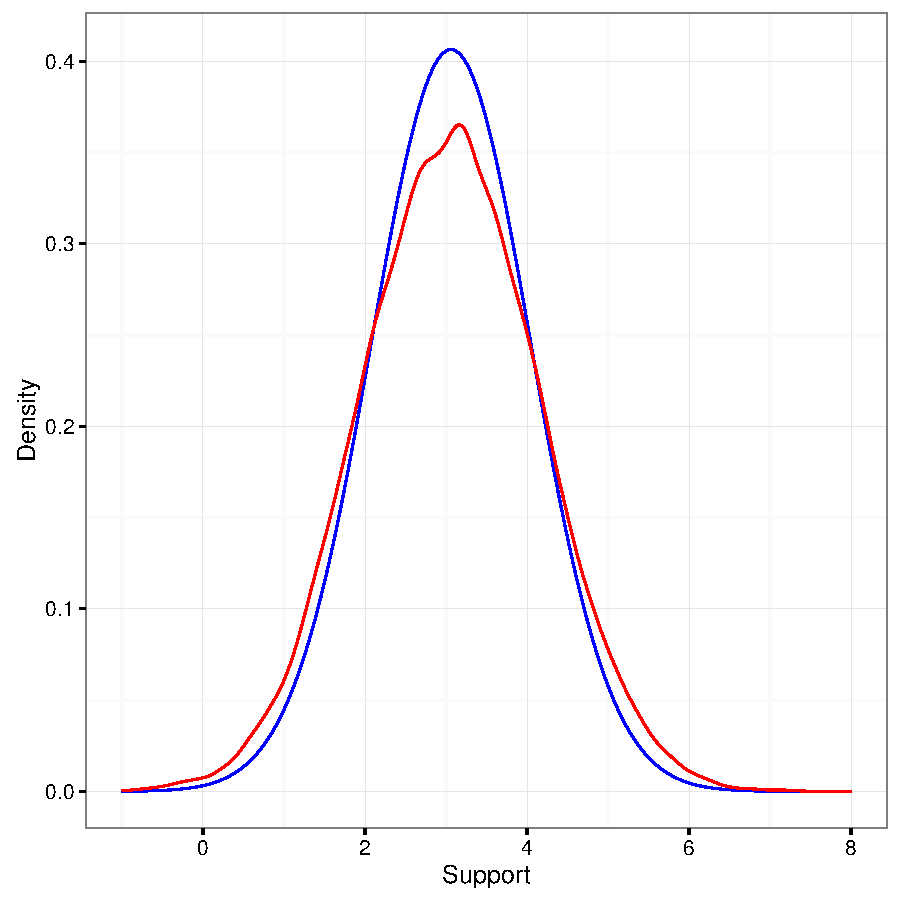
\includegraphics{ar1_predictive-plots}
\caption{Variational approximation for $q(y_{T+1}|y_{1:T})$ (blue) and the MCMC density for $p(y_{T+1}|y_{1:T})$ (red). 
The KL Divergence from q to p is 0.015, and from p to q is 0.018.}
\label{densities}
\end{figure}

\end{document}
